%%%%%%%%%%%%%%%%%%%%%%%%%%%%%%%%%%%%%%%%%%%%%%%%%%%%%%%%%%%%%%%%%%%%
%%%%%%%%%%%%%%%%%%%%%%%%%%%%%%%%%%%%%%%%%%%%%%%%%%%%%%%%%%%%%%%%%%%%
%%                                                                %%
%% An example for writting your thesis using LaTeX                %%
%% Original version by Luis Costa,  changes by Perttu Puska       %%
%% Support for Swedish added 15092014                             %%
%%                                                                %%
%% This example consists of the files                             %%
%%         thesistemplate.tex (versio 2.01)                       %%
%%         opinnaytepohja.tex (versio 2.01) (for text in Finnish) %%
%%         aaltothesis.cls (versio 2.01)                          %%
%%         kuva1.eps                                              %%
%%         kuva2.eps                                              %%
%%         kuva1.pdf                                              %%
%%         kuva2.pdf                                              %%
%%                                                                %%
%%                                                                %%
%% Typeset either with                                            %%
%% latex:                                                         %%
%%             $ latex opinnaytepohja                             %%
%%             $ latex opinnaytepohja                             %%
%%                                                                %%
%%   Result is the file opinnayte.dvi, which                      %%
%%   is converted to ps format as follows:                        %%
%%                                                                %%
%%             $ dvips opinnaytepohja -o                          %%
%%                                                                %%
%%   and then to pdf as follows:                                  %%
%%                                                                %%
%%             $ ps2pdf opinnaytepohja.ps                         %%
%%                                                                %%
%% Or                                                             %%
%% pdflatex:                                                      %%
%%             $ pdflatex opinnaytepohja                          %%
%%             $ pdflatex opinnaytepohja                          %%
%%                                                                %%
%%   Result is the file opinnaytepohja.pdf                        %%
%%                                                                %%
%% Explanatory comments in this example begin with                %%
%% the characters %%, and changes that the user can make          %%
%% with the character %                                           %%
%%                                                                %%
%%%%%%%%%%%%%%%%%%%%%%%%%%%%%%%%%%%%%%%%%%%%%%%%%%%%%%%%%%%%%%%%%%%%
%%%%%%%%%%%%%%%%%%%%%%%%%%%%%%%%%%%%%%%%%%%%%%%%%%%%%%%%%%%%%%%%%%%%

%% Uncomment one of these:
%% the 1st when using pdflatex, which directly typesets your document in pdf (use jpg or pdf figures), or the 2nd when producing a ps file (use eps figures, don't use ps figures!).
\documentclass[english,12pt,a4paper,pdftex,sci,utf8]{aaltothesis}
%\documentclass[english,12pt,a4paper,dvips]{aaltothesis}

%% To the \documentclass above:
%% specify your school: arts, biz, chem, elec, eng, sci
%% specify the character encoding scheme used by your editor: utf8, latin1

%% Use one of these if you write in Finnish (see the Finnish template):
%\documentclass[finnish,12pt,a4paper,pdftex,elec,utf8]{aaltothesis}
%\documentclass[finnish,12pt,a4paper,dvips]{aaltothesis}

\usepackage{graphicx}

%% Use this if you write hard core mathematics, these are usually needed
\usepackage{amsfonts,amssymb,amsbsy,csquotes}

% \usepackage[backend=biber,natbib=true,style=numeric-comp,sorting=none]{biblatex}
\usepackage{biblatex}
\addbibresource{./refs.bib}

%% Use the macros in this package to change how the hyperref package below typesets its hypertext -- hyperlink colour, font, etc. See the package documentation. It also defines the \url macro, so use the package when not using the hyperref package.
%\usepackage{url}

%% Use this if you want to get links and nice output. Works well with pdflatex.
\usepackage{hyperref}
\hypersetup{pdfpagemode=UseNone, pdfstartview=FitH,
  colorlinks=true,urlcolor=red,linkcolor=blue,citecolor=black,
  pdftitle={Default Title, Modify},pdfauthor={Your Name},
  pdfkeywords={Modify keywords}}


%% All that is printed on paper starts here
\begin{document}

%% Change the school field to specify your school if the automatically set name is wrong
% \university{aalto-yliopisto}
% \university{aalto University}
% \school{Sähkötekniikan korkeakoulu}
% \school{School of Electrical Engineering}

%% Only for B.Sc. thesis: Choose your degree programme.
%\degreeprogram{Electronics and electrical engineering}

%% ONLY FOR M.Sc. AND LICENTIATE THESIS: Specify your department,
%% professorship and professorship code.
\department{Department of Computer Science}
\professorship{Computer Science}
%%

%% Valitse yksi näistä kolmesta
%%
%% Choose one of these:
%\univdegree{BSc}
\univdegree{MSc}
%\univdegree{Lic}

%% Your own name (should be self explanatory...)
\author{Aarni Halinen}

%% Your thesis title comes here and again before a possible abstract in
%% Finnish or Swedish . If the title is very long and latex does an
%% unsatisfactory job of breaking the lines, you will have to force a
%% linebreak with the \\ control character.
%% Do not hyphenate titles.
%%
\thesistitle{Kubernetes inter-pod container isolation}

\place{Espoo}

%% For B.Sc. thesis use the date when you present your thesis.
\date{1.6.2023}

%% B.Sc. or M.Sc. thesis supervisor
%% Note the "\" after the comma. This forces the following space to be a normal interword space, not the space that starts a new sentence.
%% This is done because the fullstop isn't the end of the sentence that should be followed by a slightly longer space but is to be followed by a regular space.
\supervisor{Prof.\ Mario Di Francesco} %{Prof.\ Pirjo Professori}

%% B.Sc. or M.Sc. thesis advisors(s). You can give upto two advisors in this template. Check with your supervisor how many official advisors you can have.
\advisor{M.Sc.\ (Tech.)\ José\ Luis\ Martin\ Navarro}
\advisor{M.Sc.\ (Tech.)\ Jacopo\ Bufalino}

%% Aalto logo: syntax:
%% \uselogo{aaltoRed|aaltoBlue|aaltoYellow|aaltoGray|aaltoGrayScale}{?|!|''}
%%
%% Logo language is set to be the same as the document language.
%% Logon kieli on sama kuin dokumentin kieli
\uselogo{aaltoRed}{''}

%% Create the coverpage
\makecoverpage

%% Note that when writting your master's thesis in English, place
%% the English abstract first followed by the possible Finnish abstract

%% English abstract.
%% All the information required in the abstract (your name, thesis title, etc.)
%% is used as specified above.
%% Specify keywords
\keywords{Kubernetes, Container, Docker, Security}
%% Abstract text
\begin{abstractpage}[english]
  Your abstract in English. Try to keep the abstract short; approximately
  100 words should be enough. The abstract explains your research topic,
  the methods you have used, and the results you obtained.
  Your abstract in English. Try to keep the abstract short; approximately
  100 words should be enough. The abstract explains your research topic,
  the methods you have used, and the results you obtained.

  Your abstract in English. Try to keep the abstract short; approximately
  100 words should be enough. The abstract explains your research topic,
  the methods you have used, and the results you obtained.
  Your abstract in English. Try to keep the abstract short; approximately
  100 words should be enough. The abstract explains your research topic,
  the methods you have used, and the results you obtained.
\end{abstractpage}

%% Force a new page so that the possible English abstract starts on a new page
\newpage
%
%% Abstract in Finnish.  Delete if you don't need it.
% \thesistitle{Opinnäyteohje}
% \advisor{TkT Olli Ohjaaja}
% \degreeprogram{Electronics and electrical engineering}
% \department{Radiotieteen ja -tekniikan laitos}
% \professorship{Piiriteoria}
% %% Avainsanat
% \keywords{Vastus, Resistanssi,\\ Lämpötila}
% %% Tiivistelmän tekstiosa
% \begin{abstractpage}[finnish]
%   Tiivistelmässä on lyhyt selvitys (noin 100 sanaa)
%   kirjoituksen tärkeimmästä sisällöstä: mitä ja miten on tutkittu,
%   sekä mitä tuloksia on saatu.
%   Tiivistelmässä on lyhyt selvitys (noin 100 sanaa)
%   kirjoituksen tärkeimmästä sisällöstä: mitä ja miten on tutkittu,
%   sekä mitä tuloksia on saatu.

%   Tiivistelmässä on lyhyt selvitys (noin 100 sanaa)
%   kirjoituksen tärkeimmästä sisällöstä: mitä ja miten on tutkittu,
%   sekä mitä tuloksia on saatu.
%   Tiivistelmässä on lyhyt selvitys (noin 100 sanaa)
%   kirjoituksen tärkeimmästä sisällöstä: mitä ja miten on tutkittu,
%   sekä mitä tuloksia on saatu.
%   Tiivistelmässä on lyhyt selvitys (noin 100 sanaa)
%   kirjoituksen tärkeimmästä sisällöstä: mitä ja miten on tutkittu,
%   sekä mitä tuloksia on saatu.
% \end{abstractpage}

% \newpage

\mysection{Preface}
I want to thank Professor Pirjo Professori
and my instructor Olli Ohjaaja for their
good and poor guidance.\\

\vspace{5cm}
Otaniemi, 16.1.2015

\vspace{5mm}
{\hfill Eddie E.\ A.\ Engineer \hspace{1cm}}

%% Force new page after preface
\newpage

%% Table of contents.
\thesistableofcontents

%% Symbols and abbreviations
\mysection{Symbols and abbreviations}

\subsection*{Symbols}

\begin{tabular}{ll}
$\uparrow$       & electron spin direction up\\
$\downarrow$     & electron spin direction down
\end{tabular}

\subsection*{Operators}

\begin{tabular}{ll}
$\nabla \times \mathbf{A}$              & curl of vectorin $\mathbf{A}$\\
\end{tabular}

\subsection*{Abbreviations}

\begin{tabular}{ll}
K8s         & Kubernetes \\
STRIDE      & an object-oriented analog circuit simulator and design tool \\
\end{tabular}


%% Tweaks the page numbering to meet the requirement of the thesis format:
%% Begin the pagenumbering in Arabian numerals (and leave the first page
%% of the text body empty, see \thispagestyle{empty} below).
%% Additionally, force the actual text to begin on a new page with the
%% \clearpage command.
%% \clearpage is similar to \newpage, but it also flushes the floats (figures
%% and tables).
%% There is no need to change these
\cleardoublepage
\storeinipagenumber
\pagenumbering{arabic}
\setcounter{page}{1}

%% Leave first page empty
\thispagestyle{empty}

\section{Introduction}

% The sidecar pattern allows attaching new functionality to application without modifying main application source code.

\subsection{Problem Statement}

While the sidecar pattern makes it easier to add peripheral tasks to applications, it opens up questions about application security. In Kubernetes, there is limited amount of security features available on container-level. Most of the security related policies and capabilities are defined for the Pod, which essentially means that any capability required by the main application is inherited in the sidecar. Any privilege or network policy granted for the main application can be used by the sidecar for escalation and lateral movement.

Most often, developers rely on containers by third parties for the sidecar tasks. The source code of the sidecar containers, even if it were open, can be hard or even impossible to verify for known vulnerabilities. This, combined with the limited security features for sidecars, makes any exploitable security issue in the sidecar an optimal launchpad for attack against the whole cluster. Furthermore, malicious actors can use supply chain attacks and typosquatting to trick victims into installing malicious sidecars to their clusters.

This thesis proposes a solution for limiting capabilities of sidecar without limiting those of the main container, thus extending the principle of least privilege to within the pod.

\subsection{Thesis outline}

The following chapter \ref{section-bg} gives background about containers, Kubernetes and explains their common attack vectors. It also discusses Kubernetes networking and container network interface plugins. Chapter \ref{section-methods} proposes ideas for isolating sidecars from main application container. The chapter discusses both container and networking security in the context of Kubernetes Pod. Chapter \ref{section-solution} introduces an implementation based on the findings of the previous chapter. The pros and cons of the solution are discussed in Chapter \ref{section-discussion}. Finally, Chapter \ref{section-conclusion} discusses future research and concludes the thesis.

%% In a thesis, every section starts a new page, hence \clearpage
\clearpage

\section{Background} \label{section-bg}

\subsection{Principle of least priviledge, Zero trust...}

\subsection{Microservices architecture}
\subsection{Containerization and Docker}

\begin{figure}[h!]
  \centering
  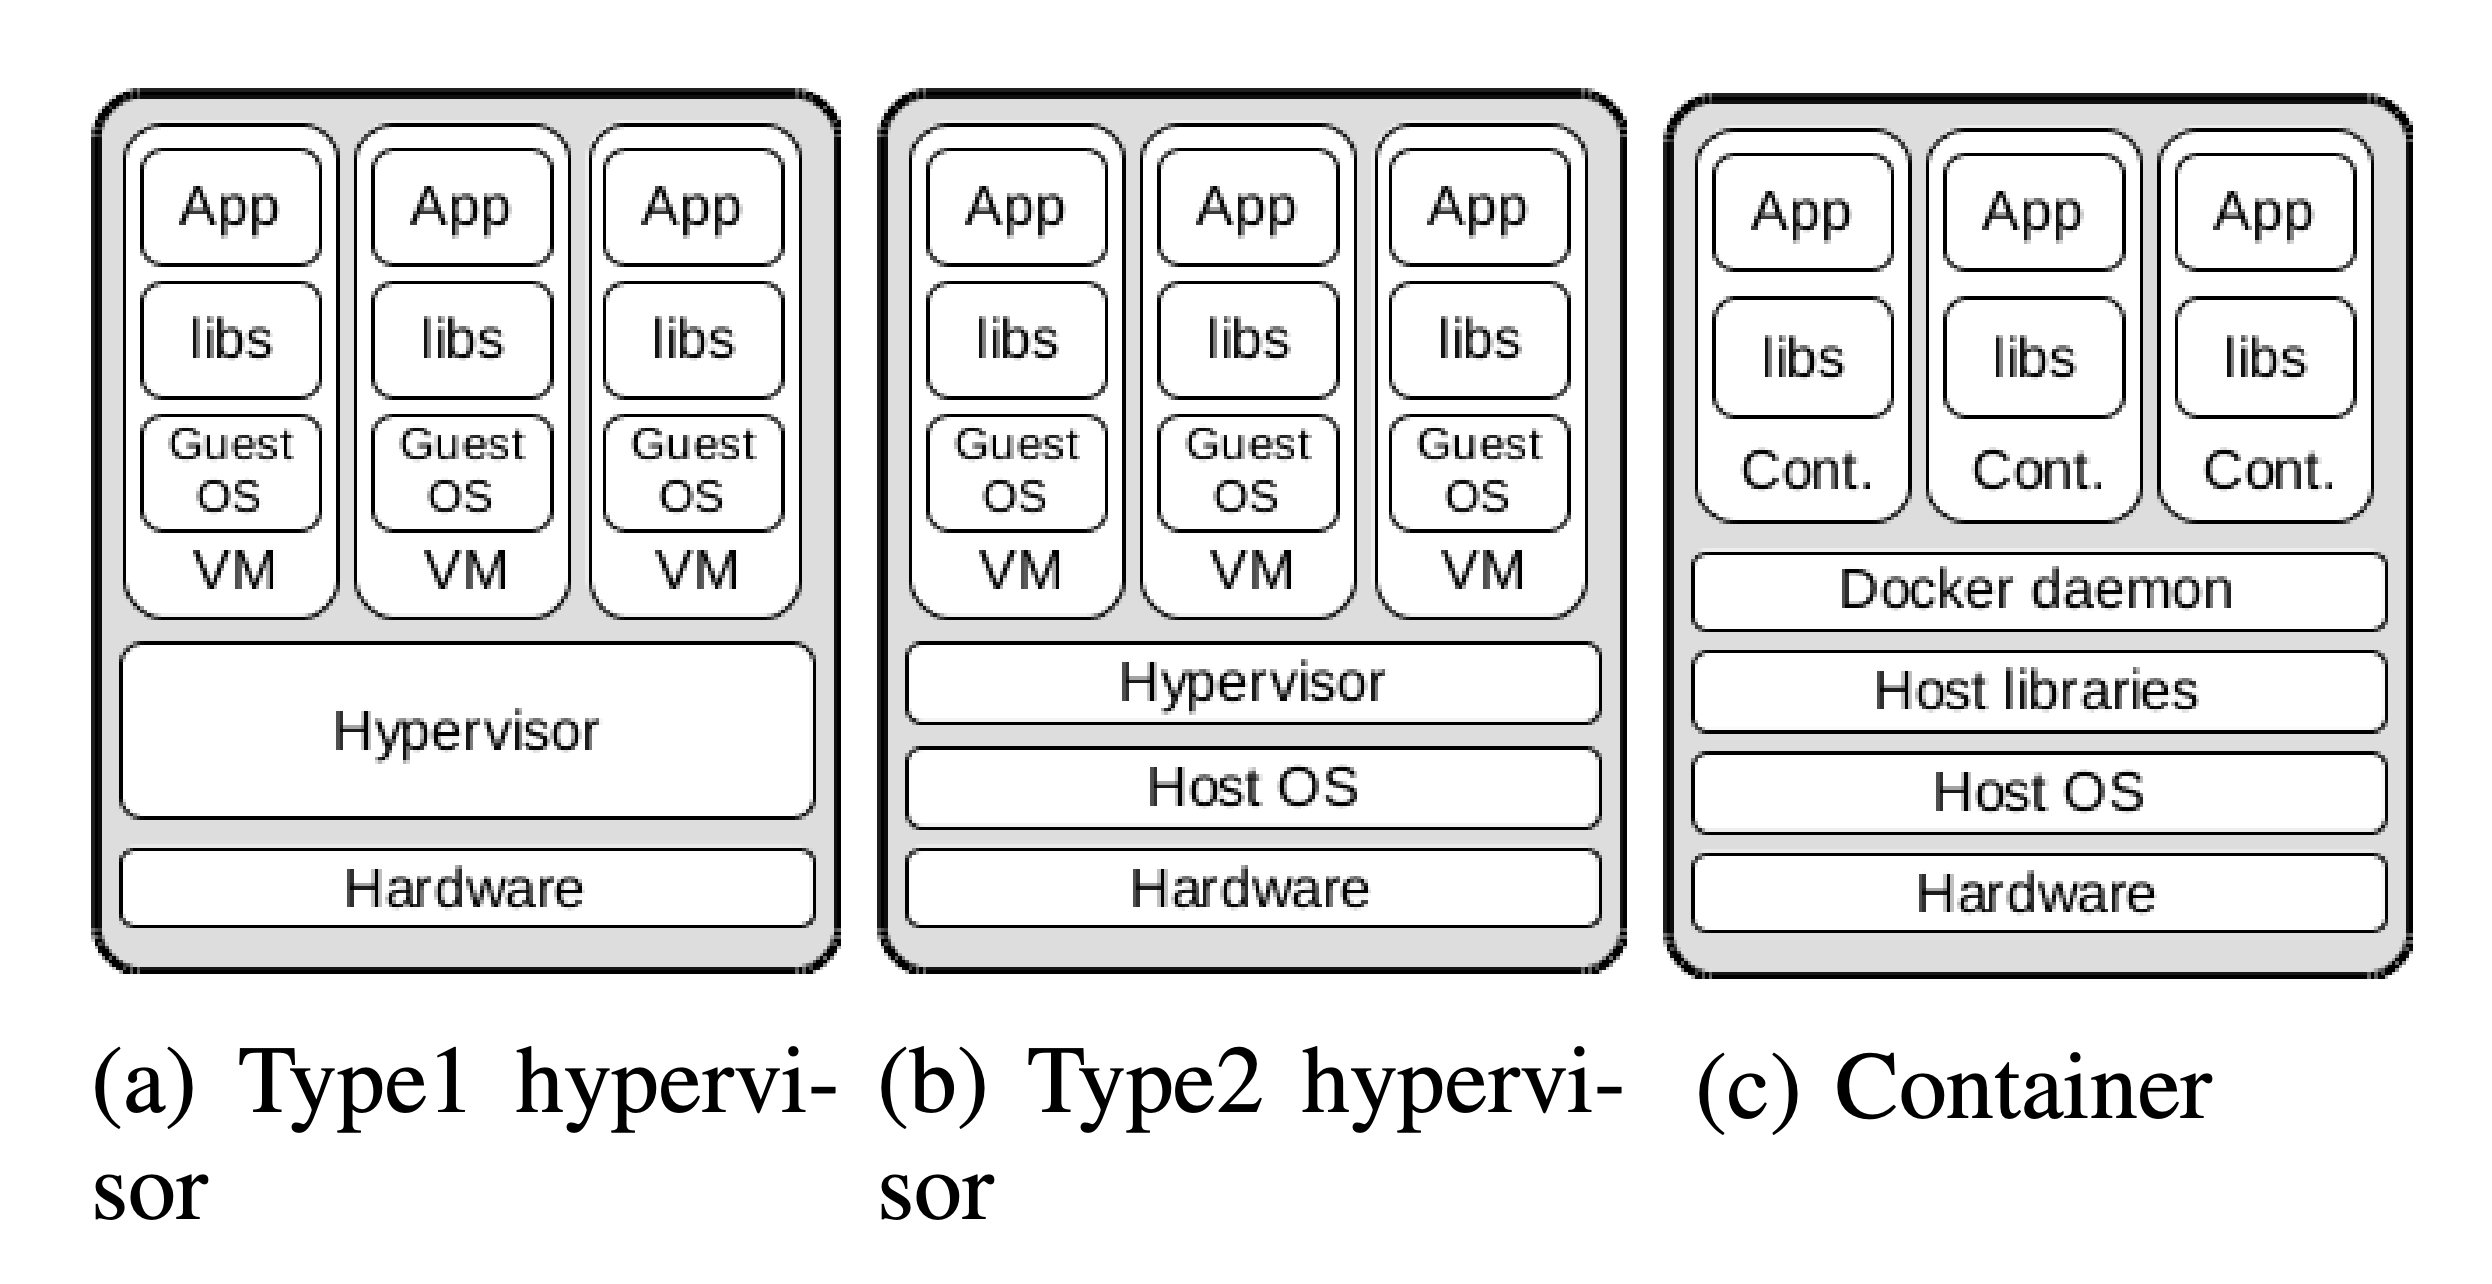
\includegraphics[width=\linewidth]{files/figure-1.png}
  \caption{Virtualization models \cite{combe2016docker}}
  \label{figure-1}
\end{figure}

Figure~\ref{figure-1} illustrates common virtualization models. Whereas traditional virtualization techniques virtualize workloads on top of a hypervisor which shares hardware resources between the virtual machines, containerization is a technique where virtualization happens on a operating system level \cite{merkel2014docker}. Processes executing in containers run on the host machine kernel. However, each container is isolated to its own network, process namespace and so on; two containers on the same host OS do not know that they share resources. Furthermore, containers are similarly isolated from accessing host OS resources.

BSD jails and \textit{chroot} can be considered early forms of containerization technology, so the idea of containers is not new \cite{combe2016docker}. Recent Linux container solutions rely on two main implementations: Linux Containers (LXC) -based solution that relies on kernel features such as control groups (cgroups) and namespaces, and a custom kernel and Linux distribution called Open Virtuozzo (OpenVZ). Docker \cite{docker} is a hugely popular container runtime that is based on LXC and provides an easy-to-use API and tooling for creating and managing containers. Docker also provides containerization for other OSes as well. However, in this thesis we focus only on the Linux implementation.

\subsubsection{Linux containers}

The Linux containers technology implements container isolation and containement using Linux kernel feature called namespaces \cite{lin2018measurement}. Namespaces \cite{manpages-namespace} are a construct that wraps a global system resource in an abstraction which makes it appear to the processes in the namespace that they have their own, isolated, instance of the global resource. There are total of eight namespaces: i) Cgroup which is used for resource management, ii) Inter-process communication (IPC) which isolates POSIX message queues etc., iii) Network which isolates network devices, stack ports etc., iv) Mount for file system isolation, v) Process ID (PID), vi) Time, vii) User for isolating user and group identifiers and viii) UTS which isolates hostnames and NIS domain names. For example, network namespace provides each container their own loopback device and even \texttt{iptables} rules. In another example, mount namespace makes sure that container has no visibility nor access to the host's or other container's file system. Compared to other namespaces that concern isolation of kernel data, cgroups focuses on limiting available system resources per namespace \cite{lin2018measurement}. Each namespace can be setup with their own limits on CPU and memory usage and available devices. Using Docker as an example, setting \textit{--cpu}, \textit{--memory} and \textit{--devices} options will limit available resources for the container.

% One critical security risk of the container mechanism is that all containers running on the same host share the same Linux kernel. If a process inside the container compromises the Linux kernel, the isolation provided by the container mechanism becomes invalid. Therefore, several Linux kernel security mechanisms are adopted to constrain the capability of the processes inside the containers, such as Capability [48], Seccomp [29] and Mandatory Access Control (MAC) mechanisms. Through Capability mechanism, the superuser privilege (i.e., ROOT privilege) is divided into 38 distinct units, known as capabilities. Each capability represents a permission to process some speci"c kernel resources. For example, the CAP_NET_ADMIN capability denotes the permissions to perform network-related operations. By default, the containers created by Docker own 14 capabilities [21]. The Seccomp mechanism constrains the system calls a process can invoke. Docker de"nes the available system calls for a container through a Seccomp pro"le "le, which by default includes more than 300 system calls [26]. Both Capability and Seccomp are Discretionary Access Control (DAC) mechanisms, and SELinux [52] and AppArmor [24] are two MAC mechanisms adopted by containers. SELinux has been integrated in CentOS / RHEL / Fedora distros, and AppArmor has been integrated in Debian/Ubuntu distros. AppArmor utilizes a path-based enforcement model [5], while SELinux adopts a label-based enforcement model [52].

Since all containers and the host machine run on same kernel, any container that manages to breakout from isolation may compromise other containers, the host and the whole kernel. To combat this container breakout, several Linux kernel security mechanisms are adopted to constrain the capabilities of containers \cite{lin2018measurement}. The mechanisms include Discretionary Access Control (DAC) mechanisms like Capability \cite{manpages-capabilities} and Secure computing mode (Seccomp) \cite{manpages-seccomp}, and Mandatory Access Control (MAC) mechanisms like Security-Enhanced Linux (SELinux) and AppArmor \cite{apparmor}. With Capability, the superuser (i.e. the root user) privilege is divided into distinct units, each of which represent a permission to process some specific kernel resources. The feature turns the binary "root/non-root" security mechanism into fine-grained access control system, which makes it easier to follow the principle of least privilege. For example, processes like web servers that just need to bind on a Internet domain privileged port (numbers less than 1024) do not need to run as root; they can just be granted with \texttt{CAP\_NET\_BIND\_SERVICE} capability instead \cite{docker-security}. The Seccomp mechanism constrains which system calls a process can invoke. The available system calls are defined for a container through Seccomp profile which is defined as a JSON file. The Docker default Seccomp profile \cite{docker-default-seccomp} includes over 300 system calls. SELinux is integrated to CentOS/RHEL/Fedora distributions and utilizes a label-based enforcement model, while AppArmor is available in Debian and Ubuntu distros and adopts a path-based enforcement model \cite{lin2018measurement}.

\subsubsection{Docker}

\begin{figure}[h!]
  \centering
  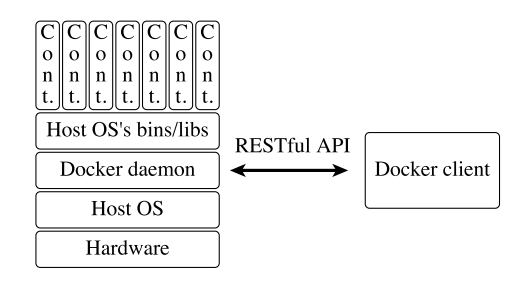
\includegraphics[width=\linewidth]{files/docker-engine.png}
  \caption{Architecture of Docker engine \cite{bui2015analysis}}
  \label{figure-docker}
\end{figure}

Docker is an open-source container technology written in Go and launched in 2013 \cite[text]{docker-what}. The platform consists of Docker Engine packaging tool, Docker image registries like the public image repository Docker Hub and Docker desktop application \cite{docker-overview}. In general, the engine architecture is similar to container-based virtualization, as visible in figure \ref{figure-docker} \cite{bui2015analysis}. The containers run on top of Docker daemon which manages and executes all the containers. The daemon is exposed to Docker clients via RESTful HTTP API. The Docker client is a command line tool which provides user interface for commanding the daemon and thus containers. By exposing the API outside the host machine, the architecture enables remote control of daemon with the client. For security reasons, remote communication should be secured with TLS.

Docker image is a read-only template with instructions for creating a Docker container \cite{docker-overview}. The images are often based on another image, such as OS images \texttt{ubuntu} and \texttt{alpine}, with some additional customizations like installation of web server binaries. The customizations are added to the image as series of data layers so that each new command creates a new layer. This process makes the distribution of image more efficient since only the changes between layers need to be distributed \cite{bui2015analysis}. The layering is achieved with special filesystem inspired by UnionFS which allows files and directories in different file systems to be combined into a single consistent file system.

Docker users can share their custom images publicly or privately in Docker Hub, or even host their own image registry platform. Most cloud providers also offer container registry services so even propietary software can be published in a private registry and used by other cloud services, like Kubernetes clusters. Whenever the image is not found locally, the client automatically tries to search and pull image from connected registries.

\subsection{Kubernetes}

Kubernetes (K8s) \cite{kubernetes} is an open-source container orchestrator, i.e. a system for automating deployment, scaling and management of containerized applications. It allows creation of a cluster which consists of a set of servers, called Nodes, on which application containers are scheduled by the system. The automation provides resilience and efficient resource utilization for workloads in the cluster: if a container or node dies, the system tries to restart and re-schedule containers so that the desired cluster state is maintained. K8s is hosted by the Cloud Nativce Computing Foundation (CNCF), but it's origins are at Google where it was created as an open-source option for Google's propietary Borg and Omega orchestrators \cite{burns2016borg}. K8s was open-sourced in 2014.

\subsubsection{Kubernetes objects}

\textbf{Pods} are the basic atomic scheduling unit in K8s. Pods consists of one or more tightly-coupled containers with shared storage volume and networking \cite{k8s-docs-pods}. Containers in a pod are always co-located and co-scheduled and run in a shared context, i.e. a set of Linux namespaces. Network, UTS and IPC namespaces are shared by default, and process namespace can be shared with \texttt{v1.PodSpec.shareProcessNamespace}. The common network namespace means that containers in a pod can communicate with each other via localhost, have common IP address and cannot re-use same port numbers. In addition to normal application container, Pods can include special \texttt{initContainers} that are only run on Pod startup. These pods are used for modifying Pod context before the actual workload starts. Multiple \texttt{initContainers} are run sequentially and a failing container blocks the execution of the following initialization and normal workloads. All Pods accross the cluster share same subnet and can access each other via IP address. However, connecting to a Pod with IP address is sub-optimal since Pods are ephermal and restarting a dead pod may receive a new IP address. Furthermore, horizontally scaled Pods with multiple replicas have as many IP addresses, thus making load balancing difficult. Kubernetes concept called Services solves these issues.

Instead of creating Pods directly, \textbf{Deployment} workload resources are used for creating Pods in a cluster, even with singleton Pods \cite{k8s-docs-pods}. With Deployments, user describes the desired state in a declarative manner. The Kubernetes control loop then creates \textbf{ReplicaSet} based on the Deployment resource, which in turn guarantees the availibility of desired amount of Pods \cite{k8s-docs-deployment}. \textbf{DaemonSet} on the other hand is a workload resource that ensures all or some Nodes run a copy of a Pod. Typical usecases for daemons are running Node monitoring and logging, and network plugins which we discuss in depth in section \ref{cni}.

\textbf{Services} are an object for exposing groups of Pods over an network \cite{k8s-docs-services}. The object defines a set of enpoints, i.e. the targeted pods, along with a policy about how to make the pods accessible. The targeted pods are determined with a \texttt{selector} field in the object specification. Meanwhile, the \texttt{type} field determines how the Service is exposed. There are four different \texttt{ServiceTypes} levels: i) the default \texttt{ClusterIP} which exposes Service inside the cluster with its own IP address, ii) \texttt{NodePort} which exposes service in each Node's IP address on static port (by default within a range of 30000-32767), iii) \texttt{LoadBalancer} which exposes the Service externally using cloud provider's load balancer and iv) \texttt{ExternalName} which is used to map Service to DNS name instead of a group of Pods. The field is designed as a nested functionality; each \texttt{ServiceType} level adds up to the previous one. Ingress object can also be used for exposing Services to outside of cluster. The Ingress object requires installation of an Ingress Controller to the cluster. Cloud providers often have their own controllers and all the examples in this thesis are executed on a local cluster where no external access is needed. Thus, the controllers are left as an exercise for the reader.

\textbf{Namespaces} provide isolation for cluster objects and allow grouping of objects under a single name. New K8s cluster starts with four namespaces: \texttt{default}, \texttt{kube-node-lease}, \texttt{kube-public} and \texttt{kube-system}. Namespaced objects like Deployments, Services and Pods are always deployed under a namespace which is \texttt{default} if not explicitly defined. \texttt{kube-system} is the namespace for all objects created by the K8s system which we focus more on the next section \ref{control-plane}. Namespaces also provide a scope for naming; names of resources need to be unique within a namespace, but not across namespaces. Namespaces are also used to enforce resource quotas, access control, and isolation for cluster users, for example in multi-tenancy setups. Pod Security Standards \cite{k8s-docs-pss}, which are used by Pod Security admission controller, are also defined at namespace level. Admission controllers are discussed in section \ref{admission-controllers}.

\subsubsection{Kubernetes components} \label{control-plane}

\begin{figure}[h!]
  \centering
  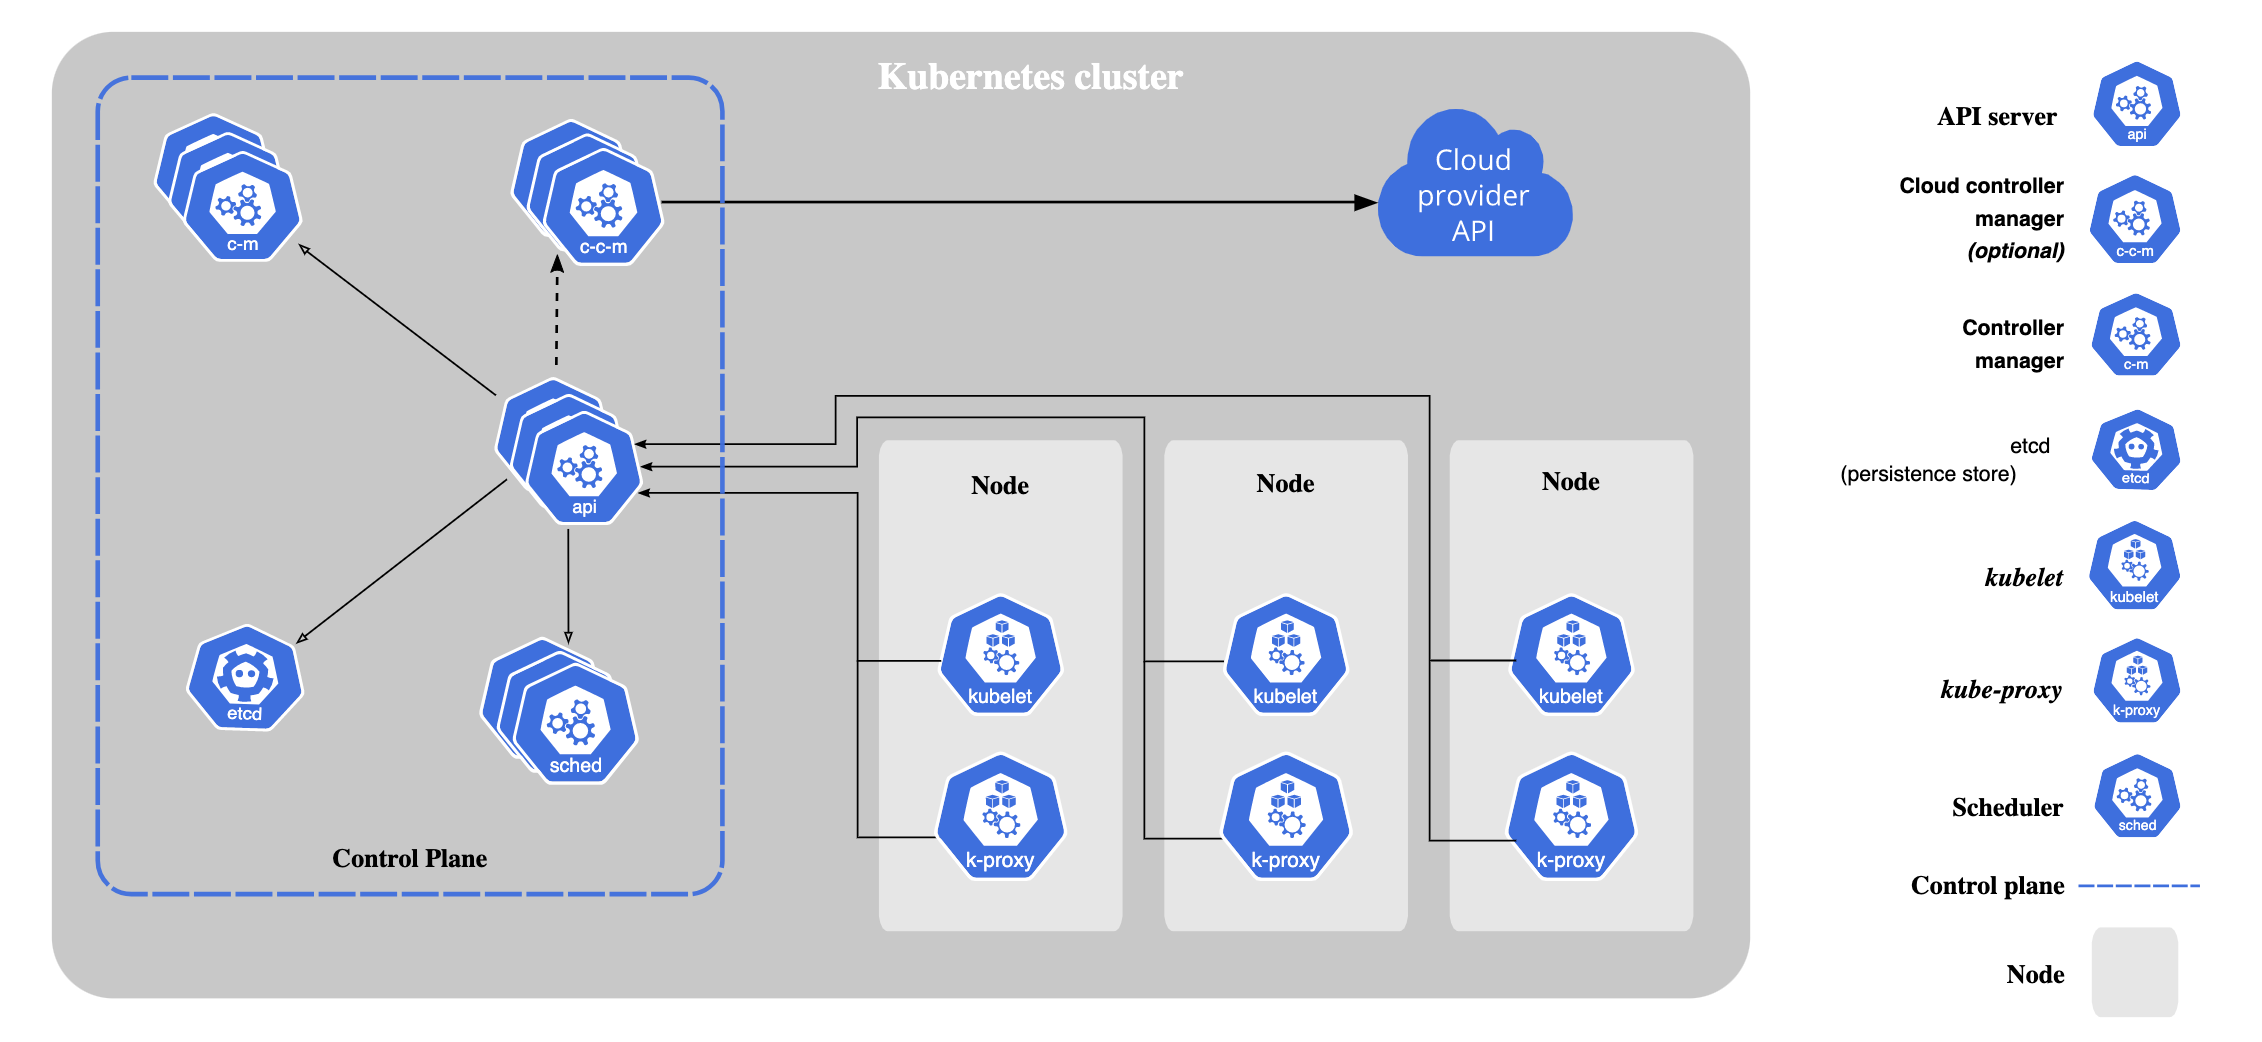
\includegraphics[width=\linewidth]{files/k8s-arch.png}
  \caption{Kubernetes cluster architecture \cite{k8s-docs-control-plane}}
  \label{figure-2}
\end{figure}

The figure \ref{figure-2} describes Kubernetes cluster with control plane and three worker nodes. The control plane consists of components that control, monitor and store the state of the cluster; essentially these are the components that are needed for complete and working Kubernetes cluster \cite{k8s-docs-control-plane}. The control plane components can be run on any worker node. However, clusters often have specialized master node for control plane components, which does not run any other containers. For fault-tolerance and high availability, control plane components should run on multiple Nodes in production environments. The control plane consists of these main components:

\textbf{API server} is a frontend component of the control plane. It is a stateless HTTP server which validates and authenticates commands given to the cluster. For valid commands, the server then forwards these to other control plane components. For example the \texttt{kubectl} CLI tool sends commands to the API server with HTTP. The main implementation of the server is \texttt{kube-apiserver}. The server can be horizontally scaled by running several instances on multiple Nodes and load balancing traffic between the instances.

\textbf{Etcd} \cite{etcd} is a strongly consistent, distributed key-value store. It is the stateful component of the control plane: all of the cluster data is stored in etcd. Thus, the stability of the component is critical for the whole cluster. To tolerate failures, etcd implements a leader-based architecture. Multiple etcd clients automaitcally elect a leader instance as the source of truth. Other instances periodically update their state from the leader instance, so that the state stays eventually conistent across all the instances. On leader failure, the other instances automatically elect new leader to keep the system functioning.

\textbf{Scheduler} watches for newly created Pods that have no assigned worker node, and selects one of the active Nodes for them to run on \cite{k8s-docs-control-plane}. The scheduling takes into account resource availibility on Nodes, Pod resource requirements, object specification affinity rules and hardware, software and policy constraints, among others.

\textbf{Controller manager} is a control plane component that runs all the controller loop processes \cite{k8s-docs-control-plane}. Controller loops, like the Deployment controller, continously watch the current and desired cluster state. When the states differ, they send commands via the API server so that the cluster moves towards the desired state. All the built-in controllers are compiled into a single binary, even though the controllers are logically different processes.

Each Node also has components that are essential for Kubernetes to work properly. \textbf{Kubelet} is an agent that makes sure containers are running in a Pod \cite{k8s-docs-control-plane}. It receives a set of pod specification from the API server and ensures that containers are running on the Node, follow the pod specifications and are healthy. Any container which is not created by Kubernetes is not managed by \texttt{kubelet}. \textbf{Kube-proxy} maintains network rules on Nodes. Part of the Serivce objects' networking is implemented by \textbf{kube-proxy}; the proxy writes \texttt{iptables} rules that route the traffic \cite{cilium-proxy-free}.

\subsubsection{Admission controllers} \label{admission-controllers}

Admission controllers are a feature of Kubernetes API server, made for  validating and modifying requests made to the server \cite{k8s-docs-admission}. The controllers execute prior to persistence of the object, but after the request is authenticated and authorized by the server. Several important features of Kubernetes are implemented with admission controllers, and these should be enabled in a properly configured API server. In addition to the built-in controllers, Kubernetes provides \texttt{MutatingAdmissionWebhook} and \texttt{ValidatingAdmissionWebhook} controllers for building own admission logic.

Admission controllers can be validating, mutating, or both \cite{k8s-docs-admission}. Mutating controllers may modify related objects to the requests they admit, while validating controllers either approve or reject the request. The control process executes mutating controllers first so that no mutations happen after the validation. If a controller in either phase rejects the request, the request is not processed further and error is returned to the end-user.

The important Admission controller for the scope of this thesis is the \texttt{PodSecurity} controller. The admission controller validates Pods before they are admitted, making sure that the requested Pod security context and other restrictions are permitted in the namespace that the Pod is assigned to \cite{k8s-docs-admission}. The controller is enabled by default, and can be taken into use just by configuring Pod Security Admission labels for Namespace objects.

The labels use \texttt{pod-security.kubernetes.io/<MODE>: <LEVEL>} format, where MODE defines the action to be taken when the security level is violated and the LEVEL is a pre-defined Pod Security Standard level. The three available levels are \texttt{privileged}, \texttt{baseline} and \texttt{restricted} \cite{k8s-docs-pss}.

The actions available are i) \texttt{enforce}, which will reject the pod on violation, ii) \texttt{audit}, which triggers an event about the violation in the audit log, and iii) \texttt{warn}, which triggers user-facing warning about the violation \cite{k8s-docs-psa}. A namespace can configure any or all three of the available modes, and even set a different level for the modes. For example, it is possible to warn the user about security policy violation without blocking the request by setting the \texttt{warn} mode more restrictive than the \texttt{enforce}.

% https://learn.microsoft.com/en-us/azure/architecture/patterns/sidecar
\subsubsection{Sidecar pattern}

As mentioned before, Pods are the basic scheduling abstraction in Kubernetes and they support management and co-scheduling of multiple containers as an atomic unit. This co-scheduling and management of multiple symbiotic containers as a single unit enables multi-container application design patterns to emerge \cite{burns2016design}. Sidecar pattern is the most common of these design patterns. As an example of this pattern, the main application container can be a simple web server pairted with a container that collects server's log file and streams them to a centralized log management system. Another example of this pattern is Istio service mesh \cite{istio} and its Envoy proxy sidecar which routes all traffic thorugh the Istio control plane for management, observability and security reasons.

% First, the container is the unit of resource accounting and allocation, so for example a web server container’s cgroup can be configured so that it provides consistent lowlatency responses to queries, while the logsaver container is configured to scavenge spare CPU cycles when the web server is not busy. Second, the container is the unit of packaging, so separating serving and log saving into different containers makes it easy to divide responsibility for their development between two separate programming teams, and allows them to be tested independently as well as together. Third, the container is the unit of reuse, so sidecar containers can be paired with numerous different “main” containers (e.g. a log saver container could be used with any component that produces logs). Fourth, the container provides a failure containment boundary, making it possible for the overall system to degrade gracefully (for example, the web server can continue serving even if the log saver has failed). Lastly, the container is the unit of deployment, which allows each piece of functionality to be upgraded and, when necessary, rolled back, independently. (Though it should be noted that this last benefit also comes with a downside – the test matrix for the overall system must consider all of the container version combinations that might be seen in production, which can be large since sets of containers generally can’t be upgraded atomically. Of course while a monolithic application doesn’t have this issue, componentized systems are easier to test in some regards, since they are built from smaller units that can be independently tested.) Note that these five benefits apply to all of the container patterns we describe in the remainder of this paper.

In the pattern, peripheral tasks such as logging, configuration and observability are isolated from the main application into helper containers. These containers, sidecars, are tightly-coupled to the parent application container and should share the lifecycle of the parent. Even though the functionality of the sidecars could be build into the main container, there are benefits for using separate containers \cite{burns2016design}. The isolation allows tweaking of containers' cgroups so that CPU cycles can be prioritized for the main container. The isolation also provides failure containement boundary between the main and sidecar processes. Since container is also the unit of deployment, the sidecar containers could be developed, tested and deployed independently from one another. Sidecar containers can also be developed with different tools and dependencies, and in a way that they are re-usable with other application containers. However, this multiplies the amount of moving parts of the overall system, which increases the size of test matrix considering all of the container version combinations that might be seen in the production environment.

\subsection{Kubernetes network model}

% https://kubernetes.io/docs/concepts/services-networking/
% https://kubernetes.io/docs/concepts/extend-kubernetes/compute-storage-net/network-plugins/

% The key requirements of the Kubernetes network model include i) Pods are IP addressable and must be able to communicate with all other Pods (on the same or different host) without the need for network address translation (NAT), and ii) all the agents on a host (e.g., Kubelet) are able to communicate with all the Pods on that host. CNI plugins may differ in their architecture but meet the above network rules.

Integral part of Kubernetes cluster is how nodes and resources are networked together. Specifically, the networking model needs to address four different type of networking problems: i) intra-Pod (ie. container-to-container within same Pod) communication, ii) inter-Pod communication between Pods, iii) Service-to-Pod communication and iv) communication from external sources to Services \cite{k8s-docs-cluster-networking}. The model also requires that each Pod is IP addressable and can communicate with other Pods without network address translation (NAT), even when Pods are scheduled on different hosts \cite{qi2020assessing}. All agents on a host should also be able to communicate with Pods on the same host. The implementation of this model is not part of Kubernetes, but is handed to special plugins that implement Container Network Interface (CNI) specification.

\subsubsection{Container Network Interface} \label{cni}

The Container Network Interface (CNI) \cite{cni} is a networking specification, which has become de facto industry standard for container networking. It is backed by CNCF \cite{qi2020assessing}. CNI was first developed for the container runtime \texttt{rkt}, but it is supported by all container runtimes and there is a large number of implementations to choose from \cite{hausenblas2018container}. Most of the container orchestrators have adopted the specification as their networking solution. The biggest outlier is Docker Swarm, which instead implements \texttt{libnetwork} \cite{libnetwork}.

The CNI specification has five distinct definitions: i) a format for network configuration, ii) a execution protocol between the container runtimes and the plugin binary, iii) a procedure for the runtime to interpret the configuration and execute the plugins, iv) a procedure for deletegating functionality between the plugins and v) data types for plugins to return their results to the runtime \cite{cni}. The network configuration is defined as a JSON file and it includes a list of plugins and their configuration. The container runtime interprets the configuration file at plugin execution time and transforms it into a form to be passed to the plugins. The execution protocol defines a set of operations (ADD, DEL, CHECK, VERSION) for adding and removing containers from the network. The operation command, similarly to other protocol parameters, are passed to the plugins via OS environment variables. The configuration file is supplied to the plugin via stdin. On successful execution, the plugin returns the result via stdout with a return code of 0. On errors, the plugin returns a specific JSON structure error message to stderr and a non-zero return code. When the runtime mutates a container network, it results in a series of ADD, DELETE or CHECK executions. These are then executed in same order as defined in the \texttt{plugins} list, or reversed order for DELETE executions. Each plugin then returns either \texttt{Success} or \texttt{Error} JSON object. The execution of a series of operations ends when it encounters the first Error response, or when all the operations have been performed.

% When a new Pod is added, the CNI plugin coordinates with the container runtime and connects the container network namespace with the host network namespace (e.g., , veth pair), assigns a unique IP address to the new Pod, applies the desired network policies and distributes routing information to the rest of the cluster.

% https://www.tkng.io/cni/

% Connectivity - making sure that a Pod gets its default eth0 interface with IP reachable from the root network namespace of the hosting Node.
% Reachability - making sure that Pods from other Nodes can reach each other directly (without NAT).

% Connectivity requirement is the most straight-forward one to understand – every Pod must have a NIC to communicate with anything outside of its own network namespace. Some local processes on the Node (e.g. kubelet) need to reach PodIP from the root network namespace (e.g. to perform health and readiness checks), hence the root NS connectivity requirement.

% Reachability, on the other hand, may require a bit of unpacking:
% - Every Pod gets a unique IP from a PodCIDR range configured on the Node.
% - This range is assigned to the Node during kubelet bootstrapping phase.
% - Nodes are not aware of PodCIDRs assigned to other Nodes, allocations are normally managed by the controller-manager based on the --cluster-cidr configuration flag.
% - Depending on the type of underlying connectivity, establishing end-to-end reachability between PodCIDRs may require different methods:
%   - If all Nodes are in the same Layer2 domain, the connectivity can be established by configuring a full mesh of static routes on all Nodes with NextHop set to the internal IP of the peer Nodes.
%   - If some Nodes are in different Layer2 domains, the connectivity can be established with either:
%     - Orchestrating the underlay – usually done with BGP for on-prem or some form of dynamically-provisioned static routes for public cloud environments.
%     - Encapsulating in the overlay – VXLAN is still the most popular encap type.

The CNI plugin must provide at least connectivity and reachability for the containers \cite{cni-tkng}. For connectivity, each Pod must have a NIC for communication outside its networking namespace. The NIC must have IP address reachable from the host Node, so that cluster processes like Kubelet health and readiness checks can reach the Pod. Reachability means that all Pods can be reached from other Nodes directly without NAT. Thus, each Pod receives an unique IP address from the \texttt{PodCIDR} range configured on the Node by the Kubelet bootstrapping phase. The end-to-end reachability between different Node \texttt{PodCIDR}s is established by encapsulating in the overlay network (for example with VXLAN) or orchestrating on the underlay network, e.g. with Border Gateway Protocol (BGP).

% Kubernetes Network Policy is the means to enforce rules
% indicating which network traffic is allowed and which Pods
% can communicate with each other. The policies applied to Pod
% network traffic can be based on their applicability to ingress
% traffic (entering the Pod) and egress traffic (outgoing traffic).
% The control strategies include “allow” and “deny”. By default,
% a Pod is in a non-isolated state. Once a network policy is
% applied to a Pod, all traffic that is not explicitly allowed will
% be rejected by the network policy. However, other Pods that do
% not have network policies applied to them are not affected. CNI
% plugins in Kubernetes can implement elaborate traffic control
% and isolation mechanisms.

% Network policies help to provide the guardrails needed to
% restrict traffic between pods (in and/or across namepaces) as
% well as between pods and external networks, by explicitly
% specifying allowed and denied connections. A network policy
% specification consists of a podSelector to specify pods
% that will be subject to the policy and policyTypes to
% specify the types of policies, i.e., ingress and/or egress. Ingress
% rules specify allowed inbound traffic to the target pods, and
% egress rules specify allowed outbound traffic from the target
% pods. Each rule is comprised of a NetworkPolicyPeer
% for selecting pods on the other side of the connection to/from
% which traffic is allowed, through a Classless Inter-Domain
% Routing (CIDR) notation that specifies IP address blocks,
% namespaces, or pod labels; and a NetworkPolicyPort
% that allows to explicitly specify ports or protocols that may
% communicate with the pod. Network policies are additive, and
% if multiple policies select a pod, traffic is restricted to what is
% allowed by the union of those policies’ ingress/egress rules.

Since Kubernetes does not provide networking between the Pods, it has no capabilities to enforce network isolation between workloads. Thus, another key feature for CNI plugins is enforcing network traffic rules. Kubernetes provides a common object called \texttt{NetworkPolicy} for CNI plugins to consume. The NetworkPolicy specification consists of a \texttt{podSelector} that specifies pods that are subject to the policy and \texttt{policyTypes} to specify Ingress and Egress rules for the traffic \cite{budigiri2021network} to the target Pod. Each rule includes \texttt{to} or \texttt{from} field for selecting Pod, Namespace or IP address block in CIDR notation on the other side of the connection, and \texttt{ports} field for explicitly specifying which ports and protocols are part of the rule. The policies are additive; when multiple rules are defined for a Pod, the traffic is restricted to what is allowed by the union of the policies. Many CNI plugins also introduce Custom Resource Definitions for their own, more granular, network policy rules.

While all CNI plugins meet the requirements listed above, they may differ in architecture significantly. The plugins can be classified based on which OSI model network layers they operate on, which Linux kernel features they use for packet filtering and which encapsulation and routing model they support for inter-host and intra-host communication between Pods. In this thesis, we focus on three different CNI plugins: Calico, Cilium and Multus.

% TODO: CNI plugins, daemons and binary \cite{qi2020understanding}.

% Src: https://www.youtube.com/watch?v=0jJBUdYOmRU
% Configurations in /etc/cni/net.d on nodes
% Kubelet monitors the directory, no need to restart it when installing CNI

\subsubsection{Calico}

Calico \cite{calico} is an open-source CNI plugin with modular architecture that supports wide range of deployment options. Each Pod created to the Calico network receives one end of a virtual ethernet device link as its default \texttt{eth0} network interface, while other end is left dangling on the host Node \cite{calico-tkng}. The Pod end of the link receives IP address from Pod CIDR, but the Node end does not. Instead, a \texttt{proxy\_arp} flag is set on the on the host side of the interface while containers have a route to link-local address \texttt{169.254.1.1}, thus making the host behave like a gateway router. For routing packets between Nodes, Calico creates a VXLAN overlay network. Optionally, Calico supports IP-in-IP overlay or non-overlay network with BGP protocol.

On each Node, a \texttt{calico-node} daemon setups CNI plugin, IPAM and possible eBPF programs. The daemon subscribes to Kubernetes API for Pod events and manages both container and host networking namespaces. Calico also deploys a single-container \texttt{calico-kube-controllers} Pod into the Kubernetes control plane. The container executes a binary that consists of controller loops for Namespace, NetworkPolicy, Node, Pod and ServiceAccount Kubernetes objects. The Calico project also introduces own CLI tool, called \texttt{calicoctl} \cite{calicoctl}, for managing Calico's custom resources. The tool provides extra validation for the resources which is not possible with \texttt{kubectl}.

Calico supports Kubernetes NetworkPolicies as well as its own namespaced \\\texttt{projectcalico.org/v3.NetworkPolicy} Custom Resource Definition (CRD). Both of the policies work on OSI layers L3 (identity, e.g. IP address) and L4 (ports). Compared to the built-in policy, the Calico policy includes features such as policy ordering, log action in rules, more flexible matching criteria (e.g., mathcing on ServiceAccounts) \cite{calico-network-policy}. The policy can also match on other Calico CRDs such as \textbf{HostEndpoints} and \textbf{NetworkSets}, which allows implementing rules on host interfaces and non-Kubernetes resources. If Calico is installed along Istio service mesh, the Calico Network Policy can enforce L7 (e.g. HTTP methods and URL paths) policies on the Envoy proxy. For policies that are not tied to a Kubernetes namespace, Calico provides a \texttt{GlobalNetworkPolicy} CRD.

\subsubsection{Cilium}

Cilium \cite{cilium} is one of the most advanced and powerful CNI plugins for Kubernetes. Similarly to Calico, it creates virtual ethernet device for each Pod and sets one side of the link into Pod's network namespace \cite{cilium-tkng} as the default interface. Cilium then attaches extended Berkeley Packet Filter (eBPF) programs to ingress traffic control (\texttt{tc}) hooks of these virtual ethernet devices for intercepting all incoming packets from the Pod. The packets are intercepted and processed before the network stack and thus \texttt{iptables}, reducing latency 20\%-30\% and even doubling the throughput of packets in some scenarios \cite{budigiri2021network}. The network between Pods running on different hosts is handled by default with VXLAN overlay, but there is support for Geneve interfaces and native-routing with BGP protocol as well \cite{cilium}.

The Cilium system consists of an agent (\texttt{cilium-agent}) daemon running on each Node, one or more operator (\texttt{cilium-operator}) Pods and a CLI client (\texttt{cilium}) \cite{cilium-components}. The agent daemons subscribe to events from Kubernetes API and manage containers' networking and eBPF programs. The CLI tool, which is installed on each agent, interacts with the REST API of the agent and allows inspecting the state and status of the local agent. The tool should not be confused with Cilium management CLI tool, also incidentally named \texttt{cilium}, which is typically installed remote from the cluster. The operator is responsible for all management operations which should be handled once for the entire cluster, rather than once for each Node. This includes for example registering of CRDs.

% TODO: Move OSI layer to somewhere else
While default Kubernetes Network Policy provides security on OSI layers L3 and L4, Cilium provides CRDs that also support for L7 policies \cite{cilium-policy-language}. If L7 policies exist, the traffic is directed to Envoy instance bundled into the agent Pod which filters the traffic. Unlike on layers 3 and 4, policy violation does not result in dropped packet but an application protocol specific denied message. For example, HTTP traffic is denied with \texttt{HTTP 403 Forbidden} and DNS requests with \texttt{DNS REFUSED}. Cilium provides \texttt{CiliumNetworkPolicy} CRD that supports all L3, L4 and L7 policies. Cilium also provides \texttt{CiliumClusterwideNetworkPolicy} custom resource which is used to apply network rules to every namespace in the cluster or even to nodes when using \texttt{nodeSelector}.

As even more advanced features, Cilium also includes natively \texttt{kube-proxy} replacement, encryption for Cilium-managed traffic and Service Mesh, among others. By default, \texttt{kube-proxy} uses \texttt{iptables} to route the Service traffic \cite{cilium-proxy-free}. With \texttt{kubeProxyReplacement} installation option, Cilium implements Service load-balancing as XDP and TC programs on Node network stack. For encryption, Cilium supports both IPsec and WireGuard implementations \cite{cilium-encryption}. The Service mesh performs variety of features directly in eBPF, thus functioning without sidecar containers or proxying requests through the agent Pod's Envoy \cite{cilium-service-mesh}. Since all features are not available as eBPF programs or on all kernel versions,  Cilium automatically probes the underlying kernel and automatically reverts to Envoy proxy when needed. For capabilities beyong the built-in mesh, Cilium also provides an integration with Istio.

% \begin{itemize}
  % \item More on network rules (probes and uses most recent features from Kernel)
  % \item Transparent encryption https://docs.cilium.io/en/v1.13/security/threat-model/
  % \item Security on different levels: https://docs.cilium.io/en/v1.13/security/network/intro/
  % \item Cilium Service Mesh https://isovalent.com/blog/post/cilium-service-mesh/
  % \item Kube-proxy replacement
  % \item Cilium components (Agent (includes Envoy), client, operator, plugin). Hubble?
% \end{itemize}

\subsubsection{Multus}

Traditionally CNI plugins only provide a single network interface for a Pod, apart from loopback device. Multus \cite{multus-cni} is a CNI plugin that allows attaching multiple network interfaces for a Pod. It does not provide any connectivity or reachability for the containers like other plugins. Instead, it is installed as the first plugin in the CNI plugin chain. When executed, the plugin delegates interface creation to other installed plugins. Since Multus does not provide any networking and thus does not independently, it is often called "meta plugin" to distinguish it from common CNI plugins like the previous Calico and Cilium.

Multus system includes a binary, a CNI configuration file and a namespaced \texttt{NetworkAttachmentDefinition} CRD that is used to define network interfaces used in Pods. The binary and the configuration file are often installed to cluster Nodes via a DaemonSet. The daemon consists of an \textit{initContainer} that copies the binary into the \texttt{/opt/cni/bin} directory, and a daemon container that setups the configuration file and optionally spawns a HTTP server for additional features such as metrics \cite{multus-cni}. The configuration file satisfies the CNI specification with few extra attributes of which the combination of \texttt{clusterNetwork} and \texttt{defaultNetworks} or \texttt{delegates} are imperative for the CNI plugin to function \cite{multus-cni-config}. The \texttt{clusterNetwork} specifies the main network of the cluster, which implements the \texttt{eth0} interface and Pod IP address. The \texttt{defaultNetworks} is an optional array of networks that should be added for any Pods by default. The values can be names of the \texttt{NetworkAttachmentDefinition} objects or paths to CNI plugin's JSON configuration files. Optionally, the \texttt{delegates} attribute can be used; it supports similar format of values. In this scenario, the first element of the array functions as \texttt{clusterNetwork} and the rest are infered as \texttt{defaultNetworks}.

% TODO: Add examples of NetworkAttachmentDefinition and Pod annotations

Attaching additional interfaces to workloads is most often configured by adding a special annotations field \texttt{k8s.v1.cni.cncf.io/networks} to workload resource definitions. In the simplest configuration, the field takes a comma-separated list of \texttt{NetworkAttachmentDefinition} names as input. The network interface identifiers can be modified by giving the attachment input in \textit{name@interface-identifier} format. Otherwise, Multus names the interfaces \textit{net0}, \textit{net1} and so on. If extra configuration for the networks is needed, the annotation also supports a JSON array format.

\subsubsection{Extended Berkeley Packet Filter}

Berkeley Packet Filter (BPF, or nowadays often cBPF) was originally developed in early 1990s as a high-performance tool for user-space packet captures \cite{mccanne1993bsd}. BPF works by deploying the filtering part of the application, \texttt{packet filter}, in the kernel-space as an agent. The \texttt{packet filter} is provided with a program (often denoted as BPF program) consisting of BPF instructions, which works as a set of rules for selecting which packets are of interest in the user-space application and should be copied from kernel-space to user-space. The instuctions are executed in a register-based pseudo machine. Since network monitors are often interested only in subset of network traffic, this limits the number of expensive copy operations across the kernel/user-space protection boundary only to packets that are of interest in the user-space application. A notable usecase for BPF is \textit{libpcap} library, which is used by network monitoring tool called \texttt{tcpdump}.

Later in the 2010s the Linux community realized that BPF and it's ability to instrument the kernel could benefit other areas than packet filtering as well \cite{vieira2020fast}. This reworked version of BPF was first merged in to Linux kernel in 2014 and is publicly called extended Berkeley Packet Filter (eBPF) to distinguish it from the original cBPF. The kernel development community continues to call the newer version BPF, but instead of the original acronym consider it a name of a technology. Similarly to the kernel community, the term BPF always refers to the eBPF in this thesis.

The eBPF programs are compiled to bytecode and loaded to kernel with \texttt{bpf()} system call \cite{miano2021framework}. Most often programs are written in restricted C and compiled with LLVM Clang compiler to bytecode. It also possible to use eBPF assembly instructions and \texttt{bpf\_asm} utility for converting instructions to bytecode. eBPF programs follow a event-driven architecture: a loaded eBPF program is hooked to a particular type of event and each occurence of the event triggers the program execution.

% TODO: Yhidstä johonkin kappaleeseen
For networking purposes, there are two eBPF hooks available for intercepting and mangling, forwarding or dropping network packets: eXpress Data Path (XDP) and Traffic Control (TC) \cite{miano2021framework}. In Cloudflares DDoS testing benchmark \cite{cloudflare-xdp}, XDP program was capable to drop 10 million and TC program 2 million packets per second, while common \texttt{iptables} INPUT rule was able to drop less than one million packets per second.

XDP programs are attached to a network interface controller (NIC) and can handle only incoming packets \cite{hoiland2018express}. The programs are called directly by the NIC driver if it has XDP support, thus executing before packets enters the network stack. This skips expensive packet parsing and memory allocation operations, and allow XDP programs to run at very high throughput. Thus, even the main networking buffer \textit{skbuff} is not populated. Some SmartNICs even support offloading the program to the NIC's own processor from host CPU, improving host machine performance even further \cite{cilium-program-types}. If the driver does not support XDP, generic XDP is used and the programs run after the packet has been parsed by the network stack.

XDP programs can read and modify contents of the packets \cite{vieira2020fast}. Since the packets are not parsed the network stack, the programs have to work with raw packets and implement own parsing functionality. The program's return value determines how the packet should be processed further. With \texttt{XDP\_DROP} and \texttt{XDP\_PASS} return values, the packet can be dropped or passed further to the networking stack respectively. The packet can also be bounced back to the same NIC it arrived on with \texttt{XDP\_TX}, usually after modifying the packet contents. \texttt{XDP\_REDIRECT} is used for redirecting the packet to a different NIC, CPU or even to another socket.

TC programs are executed when both incoming and outgoing packets reach kernel traffic control function within the Linux network stack \cite{vieira2020fast}. The ingress hook executes after the packet is parsed to \textit{skbuff} but before most of the network stack. On egress the stack is traversed in reverse, thus the hook executes after most of the network stack. TC programs can read and write directly to packet in memory. Similarly to XDP programs, the return value of the program determines further processing of the packet. The packet can be passed furhter in the stack with \texttt{TC\_ACT\_OK}, dropped with \texttt{TC\_ACT\_SHOT}, or the modified packet can be redirected back to the start of the classification with \texttt{TC\_ACT\_RECLASSIFY}, among others.

\clearpage

\section{Research material and methods} \label{section-methods}

\subsection{Container breakout scenarios}

\cite{bui2015analysis}

\begin{itemize}
  \item Privileged container
  \item CAP\_SYS\_ADMIN, mounting /proc and chroot
  \item CAP\_SYS\_PTRACE, shellcode injection to running program, nc 172.17.0.1 on port running shell
  \item Mounted docker socket, creating priviledged containers
\end{itemize}

\subsection{Prevent container breakout with Pod Security Admission}

\subsection{IPTables}

\begin{itemize}
  \item If executed from containers in Pod (init, lifecycle, wrapper container), it breaks Security admission rules (root user and NET\_ADMIN)
  \item Can be executed from Node itself, using DaemonSet (sort of a CNI plugin), but a bit hacky.
  \item Use owner module for catching egress packets (userId, groupId, processId)
\end{itemize}

\subsection{eBPF program firewall}

\begin{itemize}
  \item XDP works only for ingress
  \item TC needs some way to catch egress from sidecar
\end{itemize}

\subsection{Own pod for sidecar}

\begin{itemize}
  \item Guaranteed to work, since own network namespaces. What type of issues arise from this?
  \item Need to force pods to same node, for common volumes (if using host as storage)
  \item Implementation by hand, or Admission controller that catches sidecars?
  \item Loopback is not the same anymore. DNAT that changes localhost to external? => impossible with IPTables!
\end{itemize}

\subsection{Multus}

\begin{itemize}
  \item Requires breaking sidecar pattern with multiple Pods
  \item Allows use of custom IP addresses
  \item Hard to implement between nodes, affinity rules
  \item Loopback not easy to hijack for forwarding to new IPs
\end{itemize}

\clearpage

\section{Evaluation} \label{section-solution}

\clearpage

\section{Discussion} \label{section-discussion}

\clearpage

\section{Conclusion} \label{section-conclusion}

\clearpage

%% The \phantomsection command is nessesary for hyperref to jump to the correct page, in other words it puts a hyper marker on the page.
\phantomsection

\thesisbibliography
\printbibliography

%% Appendices
\clearpage

\thesisappendix

\section{Esimerkki liitteest\"a\label{LiiteA}}

Liitteet eiv\"at ole opinn\"aytteen kannalta v\"altt\"am\"att\"omi\"a ja
opinn\"aytteen tekij\"an on
kirjoittamaan ryhtyess\"a\"an hyv\"a ajatella p\"arj\"a\"av\"ans\"a ilman liitteit\"a.
Kokemattomat kirjoittajat, jotka ovat huolissaan
tekstiosan pituudesta, paisuttavat turhan
helposti liitteit\"a pit\"a\"akseen tekstiosan pituuden annetuissa rajoissa.
T\"all\"a tavalla ei synny hyv\"a\"a opinn\"aytett\"a.


% Intro
T\"am\"an tekstin l\"ahteen\"a oleva tiedosto on opinn\"aytteen
pohja, jota voi k\"aytt\"a\"a kandidaatinty\"oss\"a, diplomity\"oss\"a ja
lisensiaatinty\"oss\"a. Tekstin
l\"ahteen\"a oleva tiedosto on kirjoitettu  \LaTeX-tiedoston rakenteen
opiskelemista ajatellen. Tiedoston kommentit sis\"alt\"av\"at
tietoa, joka on hy\"odyllist\"a opinn\"aytett\"a kirjoitettaessa.

%% Esimerkki luettelosta. Lyhyt ajatusviiva on k\"ayt\"oss\"a
%% luettelossa, ja se on pituudeltaan
%% en dash. Merkit\"a\"an latex-koodissa --.
Johdanto selvitt\"a\"a samat asiat kuin tiivistelm\"a, mutta
laveammin. Johdannossa kerrotaan yleens\"a seuraavat asiat

\begin{itemize}
\item[--]Tutkimuksen taustaa ja tutkimusaiheen yleisluonteinen esittely
\item[--]Tutkimuksen tavoitteet
\item[--]P\"a\"akysymys ja osaongelmat
\item[--]Tutkimuksen rajaus ja keskeiset k\"asitteet.
\end{itemize}

Lyhyiden opinn\"aytteiden johdannot ovat yleens\"a liian pitki\"a, joten
johdannon paisuttamista on v\"altett\"av\"a. Diplomity\"oh\"on sopii johdanto,
joka on 2--4 sivua. %% t\"ass\"a on my\"os lyhyt ajatusviiva l. en dash.
Kandidaatinty\"on johdannon on oltava diplomity\"on
johdantoa lyhyempi. Sopivasti tiivistetty johdanto ei kaipaa alaotsikoita.

% Methods

T\"ass\"a osassa kuvataan k\"aytetty tutkimusaineisto ja
tutkimuksen metodologiset valinnat, sek\"a
kerrotaan tutkimuksen toteutustapa ja k\"aytetyt menetelm\"at.

% Results

T\"ass\"a osassa esitet\"a\"an tulokset ja vastataan tutkielman alussa
esitettyihin tutkimuskysymyksiin. Tieteellisen kirjoitelman
arvo mitataan t\"ass\"a osassa esitettyjen tulosten perusteella.

Tutkimustuloksien merkityst\"a on aina syyt\"a arvioida ja tarkastella
kriittisesti.  Joskus tarkastelu voi olla t\"ass\"a osassa, mutta se
voidaan my\"os j\"att\"a\"a viimeiseen osaan, jolloin viimeisen osan nimeksi
tulee >>Tarkastelu>>. Tutkimustulosten merkityst\"a voi arvioida my\"os
>>Johtop\"a\"at\"okset>>-otsikon alla viimeisess\"a osassa.

% Evaluation

T\"ass\"a osassa on syyt\"a my\"os arvioida tutkimustulosten luotettavuutta.
Jos tutkimustulosten merkityst\"a arvioidaan >>Tarkastelu>>-osassa,
voi luotettavuuden arviointi olla my\"os siell\"a.

Opinn\"aytteen tekij\"a vastaa siit\"a, ett\"a opinn\"ayte on t\"ass\"a dokumentissa
ja opinn\"aytteen tekemist\"a k\"asittelevill\"a luennoilla sek\"a
harjoituksissa annettujen ohjeiden mukainen muotoseikoiltaan,
rakenteeltaan ja ulkoasultaan.

\clearpage

\end{document}